\documentclass[12pt]{article}
% General packages
\usepackage{amsmath, graphicx, float, tabularx, booktabs, color}
% For adjusting margin size
\usepackage[margin=1in]{geometry}
% For setting bookmarks on pdf export
\usepackage[bookmarks,bookmarksopen,bookmarksdepth=2]{hyperref}
% For codeblocks
\usepackage{listings}
\usepackage{cite}

%Define Colors
\definecolor{dkgreen}{rgb}{0,0.6,0}
\definecolor{gray}{rgb}{0.5,0.5,0.5}
\definecolor{mauve}{rgb}{0.58,0,0.82}

% Color Code
\lstset{frame=tb,
  language=ruby,
  aboveskip=3mm,
  belowskip=3mm,
  showstringspaces=false,
  columns=flexible,
  basicstyle={\small\ttfamily},
  numbers=none,
  numberstyle=\tiny\color{gray},
  keywordstyle=\color{blue},
  commentstyle=\color{dkgreen},
  stringstyle=\color{mauve},
  breaklines=true,
  breakatwhitespace=true,
  tabsize=4
}

% Image path location
\graphicspath{ {images/} }

\begin{document}

% Title information
\title{Remote Shell-Code Execution using the SLMail-5.5.0 Service}
\author{Devin Trejo \tabularnewline devin.trejo@temple.edu}
\date{\today}
\maketitle

\section{Summary}
\label{sect:summary}
Today we extend the previous experiment with probing a buffer exploit
vulnerability inside SLMail and getting the program to execute the remotely 
placed shell-code. We successfully get SLMail to open a TCP socket listening
socket on port 4444 leading to a Administrative privileged command prompt.
The shell-code is loading remotely using a Python script that creates
the specially crafted payload that contains the shell-code inside. 

\section{Introduction}
\label{sect:intro}
This project extends the last project where we explored how to take control
of the EIP register remotely using a buffer overflow exploit found in 
SLMail-5.5.0. We extend the project by using our control of the EIP register
to run a custom shell-code function that will open a TCP socket listening 
on port 4444. The TCP socket is linked to a command prompt that will allow
us to remotely take control of the server. 

\subsection{Shell-Code and Payload Construction}
\label{sec:shellcode}
Shell-code is a specially designed set of OPCODE instructions that allows
a remote user to get a server perform any set of commands. Shell-code needs
to be specially construct to be small in size and to contain no NULL (0x00)
characters. The reason null characters are not allow is due to the way 
a remote user will pass the instruction set to the remote server. Shell-code
is typically loaded onto a remote server by passing it into a input buffer
when a service requires user input. The user input is in the format of a
string that would typically be a username and/or password combination. NULL
characters in a string type signifies the end of the string. If your 
shell-code contained NULL characters it would terminate the user input string
field pre-maturely. Thus the shell-code needs to be created to not contain
any NULL characters. The shell code also needs to be small in size. It 
helps avoid detection and also ensures that your code will be saved 
completely to memory. 

Today we will use our Python script to load a shell-code instruction set
borrowed from a database of pre-constructed shell-codes provided by the
people over at `exploit-db' \cite{Muts}. The exact shell-code can be seen 
in the final Python script seen in code listing~\ref{lst:exploit}. Some 
modifications to the packing of the shell-code have been made for our 
application. First off, since our Windows 2K server is not running SP4 
we require to change the return address. From a paper published by Nelson 
Brito we are given a table of applicable return addresses for a Windows 2k 
instance running SP0 \cite{Brito2008}. Secondly, the example provided by 
`expoit-db' is using Python 2 as their scripting language. For this project 
we are using Python 3 which handles RAW byte sequences a bit differently 
than Python 2. The changes are apparent by referencing the final code in 
code listing~\ref{lst:exploit}.

\begin{figure}[ht]
    \centering
    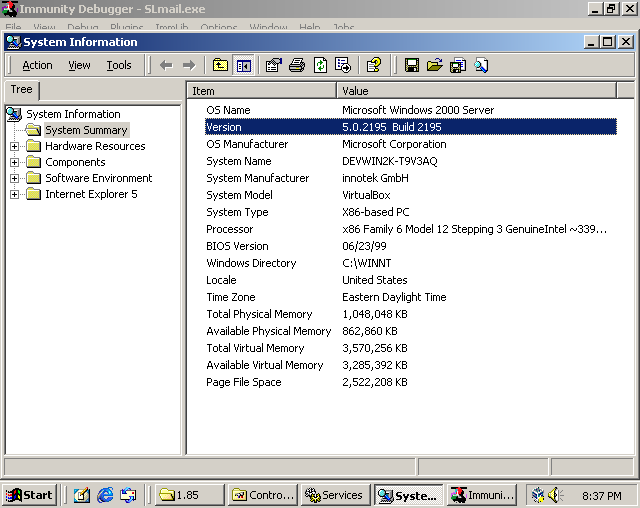
\includegraphics[width=5.5in]{images/20160504_win2ksp0.png}
    \caption{Windows 2K Server SP0 Display}
    \label{fig:win2ksp0}
\end{figure}

The result is a piece of shell-code we use will give us a remote command 
prompt with the same privileges the SLMail service runs under 
(Administrative). 

\subsection{Test Environment}
\label{sec:testenv}
As this project is an extension of the last the test environment will be 
identical as before. We use our default test environment. We have a virtual 
private network consisting of our Windows 2000 (SP0) Server 
(see figure~\ref{fig:win2ksp0}), Kali Linux penetrating machine, and a 
host machine running through Oracle Virtual Box. The virtual network has 
a DHCP server running on the VM host machine. The IP/MAC addresses for 
each are provided in table~\ref{table:pentestnetwork}.

\begin{table}[H]
    \centering
    \begin{tabularx}{\textwidth}{|*{3}{>{\centering}X|}}
        \toprule
        \textbf{Platform} & \textbf{MAC ADDR} & \textbf{Platform IPv4 Address} 
        \tabularnewline \midrule
        \textbf{Kali Linux:} & 08:00:27:94:5b:ba & 192.168.56.102 
        \tabularnewline
        \textbf{Windows 2k Server:} & 08:00:27:87:29:68 & 192.168.56.105
        \tabularnewline
        \textbf{VM Host Machine:} & 08:00:27:7c:86:0d & 192.168.56.100
        \tabularnewline \bottomrule
    \end{tabularx}
    \caption{IP Configuration for SLMail Pen-test Virtual Network}
    \label{table:pentestnetwork}
\end{table}

For the majority of the project we will be running our scripts from our VM
host machine. We use our Kali Linux solely to perform active information 
probing of the target machine. Our Windows 2K server instance will be 
be a fresh install of Windows with the only other 3rd party applications being
SLMail-5.5.0, Anaconda 2.4.0, MinGw32-1.0.0, and Immunity debugger 1.85.

\section{Discussion}
\label{sect:discussion}
To begin we perform a NMAP scan against our Windows 2K virtual machine
to show what a typical Windows instance has running by default. We know 
that our malicious shell-code will eventually open a TCP socket on port
4444 which from our initial NMAP scan seen in figure~\ref{fig:nmapwindows}
we can see in not currently open.

\begin{figure}[ht]
    \centering
    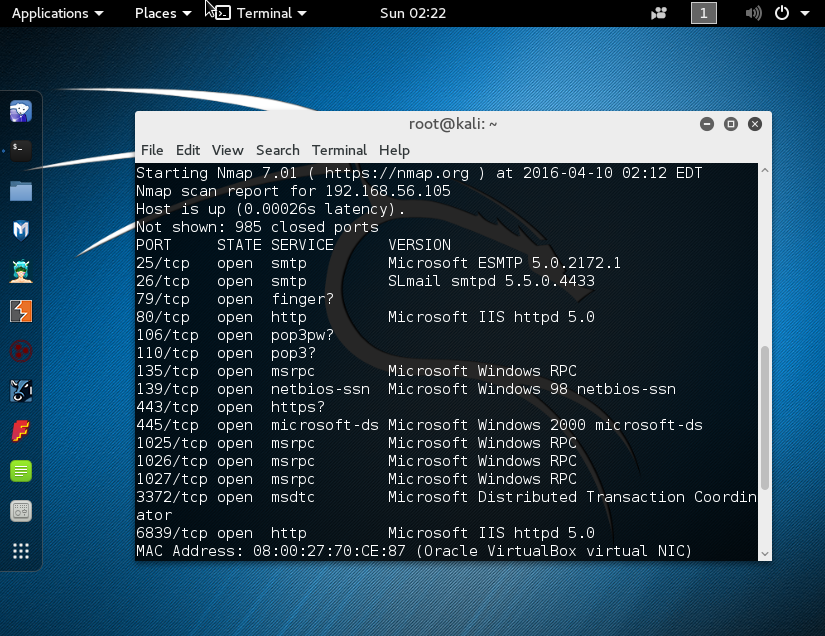
\includegraphics[width=5.5in]{images/20160504_nmap00.png}
    \caption{NMAP Scan of Windows Server 2k}
    \label{fig:nmapwindows}
\end{figure}

Now we will perform our exploit by running our Python script from our host
Arch Linux machine. The Python script we have will successfully load the 
shell-code into the remote server's memory and execute it. The shell-code 
also handles the program appropriately so that after running our malicious 
code it will not crash the SLMail service. Performing a NMAP scan after 
running our script will show that we now have a TCP socket open listening 
for connections on port 4444. 

\begin{figure}[ht]
    \centering
    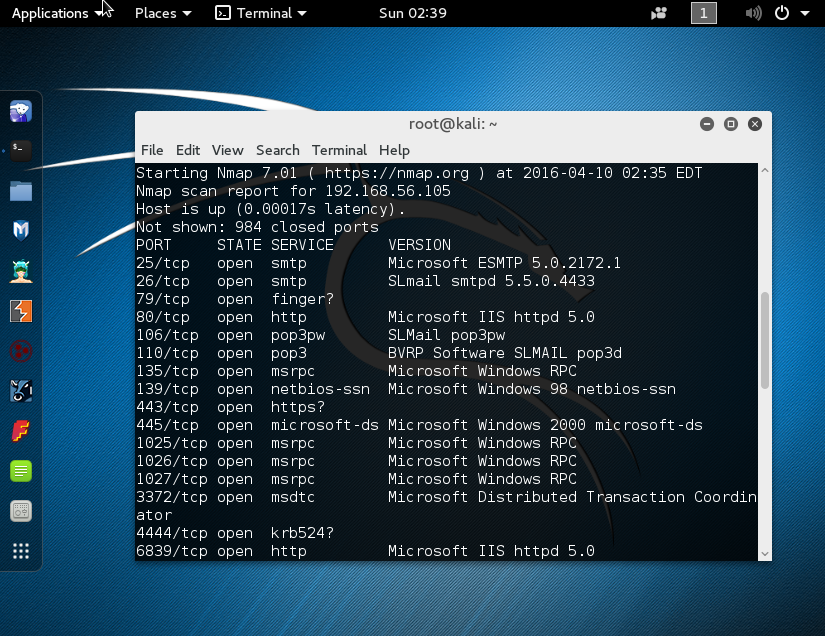
\includegraphics[width=5.5in]{images/20160504_nmap01.png}
    \caption{NMAP Scan of Windows Server 2k}
    \label{fig:nmapwindows2}
\end{figure}

At this point we can connect to the remote socket by using TELNET and
specifying a connection to our Windows 2K server over port 4444. We
will be greet by a connection successful then given control of a 
administrative Windows command prompt. The result is shown in 
figure~\ref{fig:exploited}.

\begin{figure}[H]
    \centering
    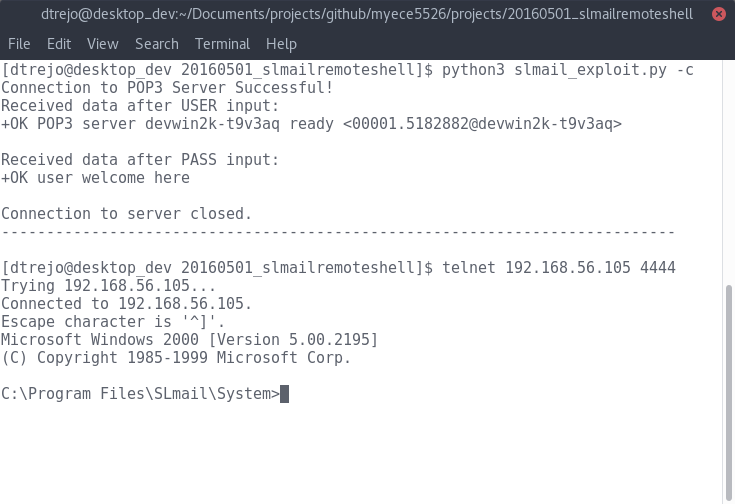
\includegraphics[width=5.5in]{images/20160504_exploited.png}
    \caption{Shell with a Successful Windows CMD}
    \label{fig:exploited}
\end{figure}

\section{Conclusion}
\label{sect:conclusion}
In this report we have demonstrated that we can take control of a remote
server by exploiting a service containing a buffer overflow vulnerability. 
The exploit is severe and shows how easy it is to get a shell that would
contain administrative privileges. A clear understanding of how compilers
create programs and how machines run the code is require in order to 
manipulate the expected function process. The takeaway from this paper is
that as a developer you need to be careful to not create any of the 
vulnerabilities. To do that, you need to understand each line of code you
right and ask yourself ``Can this line of code be exploited to do something
from its original intention?''

\nocite{*}
\bibliographystyle{IEEEtran}
\bibliography{20160504_project.bib}

\section*{Appendix}
\label{sect:appendix}
\lstinputlisting[language=Python, 
caption=SLMail Remote Shell-Code Exploit,
label=lst:exploit]{slmail_exploit.py}

\end{document}